\section{Numeric result}
\label{sec:numerical-result}
We conduct a numerical analysis to compare the proposed service and conventional mechanism. The LTE system total bandwidth is assumed to be $10$ MHz. Since there is no consensus about distribution of reporting period $T$, we thus assume that $T$ is distributed between $1$ min and $24$ hours. The number of LTE frames $W$ contained in A polling window is set as $10$. RRC inactivity timer is set as $10$ seconds. For parameters used in \eqref{eq:debit_with_respect_sinr}: bandwidth efficiency $\beta$, SNR efficiency $\Theta_{\text{ref}}$, correction factor $\eta$, they are respectively set as $0.83$, $1.25$, $1$, as in reference~\cite{mogensen2007lte}. The power compensation factor $\alpha$ is $0.1$.
The values of aforementioned system parameters are resumed in Tab.~\ref{tab:numerical-result-parameters}.

\begin{table}[]
	\centering
	\caption{Parameter Values for Numerical Results}
	\label{tab:numerical-result-parameters}
	\begin{tabular}{@{}lcc@{}}
		\toprule
		Parameter Name               & Parameter Notation    & Value                           \\ \midrule
		Reporting period             & $T$                   & $1$ min, $24$ hours \\
		Polling window               & $W$                   & $10$                            \\
		RRC inactivity timer         & $T_{\text{timer}}$    & $10$ seconds                    \\
		LTE frame duration           & $T_f$                 & $10$ ms                         \\
		Path-loss exponent           & $\gamma$              & $4.0$                           \\
		Power compensation factor    & $\alpha $             & $0.1$                           \\
		RB bandwidth                 & $B$                   & $180$ KHz                       \\
		Bandwidth efficiency         & $\beta$               & $0.83$                          \\
		SNR efficiency               & $\theta_{\text{ref}}$ & $1.25$                          \\
		Correction factor            & $\eta$                & $1.0$                           \\
		Number of served devices eNB & $N_d$                 & $20000,30000,..., 50000$        \\ \bottomrule
\end{tabular}
\end{table}


\subsection{Lower Bound of RNTI Consumption}
From Sec.~\ref{sec:lower_bound_rnti}, we observe that the lower bound of RNTI consumption, required by our proposal and the conventional LTE random access procedure, depends on the distribution of reporting period $T$. Note that the proposed polling service consumes PRD-RNTI while the conventional LTE random access mechanism use C-RNTI. Both types of RNTI are simply written as RNTI. 

The RNTI consumption comparison is conducted by supposing that $T$ follows truncated log-normal distribution and uniform distribution. Similar analysis can be made for other truncated distributions. In addition, we also do the performance analysis within a traffic model~\cite{3GPP/cellularIoT} used by 3GPP.

To cover the reporting period from $1$ min to $24$ hours, according to Eq.~\eqref{eq:period-conversion}, we obtain the eNB supported polling period list: $51.2$ sec, $102.4$ sec, $204.8$ sec, $409.6$ sec, $\cdots$, $52428.8$ sec, $104857.6$ sec (i.e.$29.13$ hour ). Polling period $T_n$ is thus a discrete random variable. The proportion of devices that use a given polling period can be determined with the PDF of $T$.

\subsubsection{Truncated log-normal distribution}
We assume that logarithm of $T$, namely $\ln T$, follows normal distribution noted as $N (\mu, \sigma^2)$. The probability of $T$ in interval $1$ min and $24$ hours is $95\%$. Thus, 
% 2015-01-10
% ln(24) = 3.18 
% ln(1.0/60) = -4.09
% ln(2.0/60) = -3.40
% u-sigma_max <= -4.09 ==> sigma_max >= 4.09 => we could take 4.2
% u-2*sigma_min <= -4.09 ==> sigma_min >= 2.04  => we could take 2.1
% 2017-08-27
% [ln(60) + ln(24*3600) ] / 2.0= mu
% mu + sigma = ln(24*3600) => sigma = 
% mu + 2*sigma = ln(24*3600) => sigma = 
$\mu = \left( \ln(60) + \ln(24*3600) \right)/2 = 7.73$, $\sigma = (\ln(24*3600) - \mu)/2 = 1.82$. To get a truncated lognormal distribution, we regard all reporting periods less than $1$ min as $1$ min and all reporting periods greater than $24$ hours as $24$ hours. 
%Therefore, the mean of reporting period $T$ is represented as shown in formula (\ref{eq:T-expectation}).
%\begin{align}
%	f_{T}(x) &= \frac{1}{\sigma \sqrt{2\pi}x} \exp -\frac{(\ln x )^2}{2\sigma^2} \nonumber \\
%	E[T] &=\frac{1}{60}P\{ T= 1 min\} + \int_{\frac{1}{60}}^{24} t \cdot f_{T}(t) dt +24P\{ T= 24 hour\} \nonumber \\
%	& = \frac{1}{60}\Phi (\frac{\ln 1/60}{\sigma}) +  \Phi (\frac{\ln 24}{\sigma}) -\Phi (\frac{\ln 1/60}{\sigma}) + 24 \cdot ( 1-\Phi (\frac{\ln 24     }{\sigma}))
%	\label{eq:T-expectation} 	
%\end{align}

% whose probability distribution is the following: 
%\begin{align}
%	& P\{ T_n = N \} = \Phi(\frac{\ln 2N}{\sigma}) - \Phi(\frac{\ln N}{\sigma}) , n=1,2...N_{max}-1 \nonumber \\
%	%						   	\shortintertext{For the minimum and maximum supported polling period:}
%	& P\{ T_0 = N \} = \Phi(\frac{\ln N}{\sigma}) \nonumber \\
%	& P\{ T_{N_{max}} = N \} = 1- \Phi(\frac{\ln N-0}{\sigma}) \nonumber 					   
%\end{align}
Given distribution of each polling period and number of MTC devices served by one eNB, the consumption of RNTI could be estimated by~\eqref{eq:lower-bound} and \eqref{eq:low-bound-rach}. The result is shown in Fig.~\ref{fig:log-normal-RNTI-consumption}.
\begin{figure}[!t]
	\centering
	\includegraphics[width=\linewidth]{Chapter6/Figures/lognorm_RNTI_consumption_comparison.eps}
	\caption{Comparison of RNTI required for case of truncated lognormal distribution}
	\label{fig:log-normal-RNTI-consumption}
\end{figure}

\subsubsection{Uniform distribution}
We suppose that $T$ follows uniform distribution between $1$ min and $24$ hours. The expectation of $1/T$ can be determined from the PDF of the considered uniform distribution . Given total device number and the repartition of each polling period, it is not difficult to get the probability distribution for each eNB supported polling period and estimate device repartition, and further estimate the minimum required RNTI for both case according to formula \eqref{eq:lower-bound} and \eqref{eq:low-bound-rach}. The comparison result is shown in Fig.~\ref{fig:uniform-RNTI-consumption}.

\begin{figure}[!t]
	\centering
	\includegraphics[width=\linewidth]{Chapter6/Figures/uniform_RNTI_consumption_comparison.eps}
	\caption{Comparison of RNTI required for case of uniform distribution}
	\label{fig:uniform-RNTI-consumption}
\end{figure}

\subsubsection{Traffic Model~\cite[Annex E]{3GPP/cellularIoT}}
In~\cite[Annex E]{3GPP/cellularIoT}, 3GPP gives a device reporting distribution to study the performance of MTC over cellular networks. It is assumed that inter-arrival time periodicity for MAR periodic is: $1$ day ($40\%$), $2$ hours ($40\%$), $1$ hour ($15\%$), and $30$ minutes ($5\%$). 

To cover the range from $30$ minutes to $24$ hours, According to Eq.~\eqref{eq:period-conversion}, the supported polling period list is $1638.4$,  $3276.8$,    $6553.6$,  $13107.2$,   $26214.4$,   $52428.8$,  $104857.6$. The RNTI consumption of two methods within such a traffic model is illustrated in Fig.~\ref{fig:3GPP_traffic_model_RNTI_consumption_comparison}. 
\begin{figure}[!t]
	\centering
	\includegraphics[width=\linewidth]{Chapter6/Figures/3GPP_traffic_model_RNTI_consumption_comparison.eps}
	\caption{Comparison of RNTI required for the traffic model proposed by 3GPP}
	\label{fig:3GPP_traffic_model_RNTI_consumption_comparison}
\end{figure}


%\subsubsection{Pareto distribution}
%We suppose that user-defined reporting period $T$ follows pareto distribution that always greater than $1$ min. The cumulative distribution function of Pareto distribution is:
%\begin{align}
%	F_T(t) = 1 - (\frac{T_{\text{min}}}{t})^{\alpha}, t \geq T_{\text{min}} 
%\end{align}
%where $\alpha$ is the shape parameter. To make sure that most values of $T$ are within $\left[1 min, 24 hours \right] $, let $T_{\text{min}}  = 60 $seconds, $\alpha = 1$. Now we can estimate $\mathbb{E}[T] = 120$ seconds.

From Fig.~\ref{fig:log-normal-RNTI-consumption}, Fig.~\ref{fig:uniform-RNTI-consumption} and Fig.~\ref{fig:3GPP_traffic_model_RNTI_consumption_comparison}, we confirm that the distribution of reporting period $T$ has a significant impact on RNTI consumption. For distribution that spreads out over the reporting range, such as uniform distribution, the RNTI consumption economization compared to the conventional LTE random access is smaller than in case where distribution is centered such as truncated lognormal distribution. No matter in which case, with less than $10$ RNTI, our proposal can serve up to $50000$ devices.

\subsection{Resource Block Pairs Consumption}
To get the exact RRC message payload size, we do a realistic measurement to capture the exchange traffic between a UE and eNB. The economized bytes number, in uplink and downlink, are resumed in Table.~\ref{tab:economized-bytes}. The bytes related to security and integrity are ignored. The PDCP protocol header occupies $1$ bytes, RLC header occupies $1$ bytes. The header of MAC layer is a little complicated. Normaly MAC header takes $2$ bytes, however, before contention resolution stage, the MAC layer should contain a random number as temporary UE identifier ($6$ bytes) and an associated subheader ($1$ bytes).

The size of data packet application layer payload is assumed to follow a truncated Pareto distribution with shape parameter $2.5$. The application payload size  range is $\left[ 20, 200\right] $ (unit bytes) , and packet header size is $29$ bytes~~\cite[Annex E]{3GPP/cellularIoT}. Thus, we assume that total data packet size varies between $\left[ 50, 230 \right] $ bytes.

\begin{table}[h]
	\centering
	\caption{RRC messages exchanged between UE and the eNB (unit: bit)}
	\label{tab:economized-bytes}
	\resizebox{0.9\textwidth}{!}{%
		\begin{tabular}{@{}lcccccc@{}}
			\toprule
			RRC Message Name                  & \thead{Payload \\Size} & \thead{MAC \\ Header} & \thead{RLC \\ Header} & \thead{PDCP \\Header} & Downlink & Uplink \\ \midrule
			ConnectionSetupRequest            & 48           & 72         & 8          & 8           &          & 136    \\
			ConnectionSetup                   & 320          & 72         & 8          & 8           & 408      &        \\
			ConnnectionSetupComplete          & 56           & 16         & 8          & 8           &          & 88     \\
			ConnectionReconfiguration         & 632          & 16         & 8          & 8           & 664      &        \\
			ConnectionReconfigurationComplete & 16           & 16         & 8          & 8           &          & 48     \\
			ConnectionRelease                 & 16           & 16         & 8          & 8           & 48       &        \\ \midrule
			Economized Bytes Number           & \multicolumn{4}{l}{}                                 & 1120     & 272    \\ \bottomrule
		\end{tabular}%
	}
\end{table}
\subsubsection{Downlink RB pairs consumption}
Only signaling messages consume RB in the downlink. We take the message RRC \emph{ConnectionReconfiguration} as example, to estimate the average amount of RB pairs are consumed within one TTI for the downlink channel in a hexagonal cell. 

The information of transport block size that one pair of RB can carry and their corresponding TBS index is taken from~\cite[Tab.~7.1.7.2.1-1]{lte-eutra-physical-layer} and placed into the left two columns in Tab.~\ref{tab:tbs-distance}. The SNR threshold and the corresponding maximum relative distance, respectively obtained from \eqref{eq:sinr_threshold} and \eqref{eq:sinr_with_repsect_distance}, are resumed in Tab.~\ref{tab:tbs-distance}. Since RRC \emph{ConnectionReconfiguration} contains $664$ bits (i.e. $83$ bytes, resumed in Tab.~\ref{tab:economized-bytes}), the required number of RB pairs is shown in the right most column of Tab.~\ref{tab:tbs-distance}).

\begin{table}
	\centering
	\caption{SNR threshold and distance for message \emph{ConnectionReconfiguration}}
	\label{tab:tbs-distance}
	\begin{tabular}{ccccc}
		\toprule
		\thead{TBS\\Index} &  \thead{TBS \\ (unit: bits)} & \thead{SINR Threshold \\(in decimal) }& \thead{Maximum \\ relative distance}&  \thead{Number of \\RB Pairs} \\
		\midrule
		    4 &   60 &           0.40 &     1.000 &     12 \\
			5 &   72 &           0.50 &     0.983 &     10 \\
			6 &   88 &           0.63 &     0.948 &      8 \\
			7 &  112 &           0.85 &     0.904 &      6 \\
			8 &  128 &           1.01 &     0.878 &      6 \\
			9 &  148 &           1.23 &     0.850 &      5 \\
			10 &  164 &           1.43 &     0.829 &      5 \\
			11 &  188 &           1.74 &     0.801 &      4 \\
			12 &  220 &           2.22 &     0.767 &      4 \\
			13 &  244 &           2.63 &     0.744 &      3 \\
			14 &  276 &           3.25 &     0.716 &      3 \\
			15 &  300 &           3.78 &     0.696 &      3 \\
			16 &  316 &           4.17 &     0.684 &      3 \\
			17 &  348 &           5.03 &     0.659 &      2 \\
			18 &  388 &           6.31 &     0.631 &      2 \\
			19 &  420 &           7.52 &     0.610 &      2 \\
			20 &  452 &           8.93 &     0.590 &      2 \\
			21 &  500 &          11.47 &     0.561 &      2 \\
			22 &  532 &          13.50 &     0.543 &      2 \\
			23 &  564 &          15.86 &     0.525 &      2 \\
			24 &  596 &          18.60 &     0.508 &      2 \\
			25 &  628 &          21.78 &     0.492 &      2 \\
			26 &  740 &          37.47 &     0.438 &      1 \\
		\bottomrule
	\end{tabular}
\end{table}

Aggregating according to the consumed RB pairs number, we obtain~Tab.~\ref{tab:RB_Distance_Interval}. According to Tab.~\ref{tab:RB_Distance_Interval}, the relative distance can be divided into a series of interval in which the eNB consume the same RB. Apply \eqref{eq:avg_RB_nb_downlink_final}, the average number of RB pairs, consumed by one device in a hexagonal cell within one TTI to transmit RRC \emph{ConnectionReconfiguration} message, is thus $2.85$.

\begin{table}
	\centering
	\caption{RB pairs number and relative distance interval for message \emph{ConnectionReconfiguration}}
	\label{tab:RB_Distance_Interval}
	\begin{tabular}{cccc}
		\toprule
		\thead{Relative Distance($r/R_{eq}$) \\ Interval }& RB \\
		\midrule
		$\left[0.000, 0.438 \right]$ &         1 \\
		$\left[0.438, 0.659\right]$  &         2 \\
		$\left[0.659, 0.744\right]$ &         3 \\
		$\left[0.744, 0.801 \right]$  &         4 \\
		$\left[0.801, 0.850\right]$  	&         5 \\
		$\left[0.850, 0.904\right]$		&         6 \\
		$\left[0.904, 0.948  \right]$	&         8 \\
		$\left[0.948, 0.983 \right]$  	&         10\\
		\bottomrule
	\end{tabular}
\end{table}



Similar methodology can be used to estimate the RB consumption for other signaling messages: $1.91$ pairs of RB for \emph{ConnectionSetup} message, $1.0$ pair of RB for \emph{ConnectionRelease}. In total, the conventional random access requires on average $5.76$ pairs of RB for downlink signaling message transmission. 

\subsubsection{Uplink RB pairs consumption}
Given a uplink reporting packet with size $100$ bytes, i.e., $800$ bits, the table indicating the SNR threshold, the maximum relative distance to the equivalent disk radius $R_{eq}$, the selected TBS index, is illustrated in Tab.~\ref{tab:uplink-tbs-distance}. Similarly, we find the RB consumption number and the distance interval and resume them into Tab.~\ref{tab:uplink_RB_Distance_Interval}. From \eqref{eq:avg_RB_nb_downlink_final}, we obtain that the uplink $100$ bytes transmission on average requires $3.31$ pairs of RBs. In term of uplink signaling, message \emph{ConnectionSetupRequest} , \emph{ConnectionSetupComplete}, \emph{ConnectionReconfigurationComplete} respectively consumes $1$ pairs of RBs.

\begin{table}
	\centering
	\caption{SNR threshold and maximum relative distance for $100$ bytes in the uplink}
	\label{tab:uplink-tbs-distance}
	\begin{tabular}{ccccc}
		\toprule
		\thead{TBS\\Index} &  \thead{TBS \\ (unit: bits)} & \thead{SINR Threshold \\(in decimal) }& \thead{Maximum \\ relative distance}&  \thead{Number of \\RB Pairs} \\
		\midrule
		6 &   88 &        0.630284 &   1.000219 &     10 \\
		7 &  112 &        0.851753 &   0.994458 &      8 \\
		8 &  128 &        1.013709 &   0.947516 &      7 \\
		9 &  148 &        1.233814 &   0.897185 &      6 \\
		10 &  164 &        1.425210 &   0.861956 &      5 \\
		11 &  188 &        1.740310 &   0.815433 &      5 \\
		12 &  220 &        2.218916 &   0.762218 &      4 \\
		13 &  244 &        2.627502 &   0.727260 &      4 \\
		14 &  276 &        3.248106 &   0.685661 &      3 \\
		15 &  300 &        3.777915 &   0.657478 &      3 \\
		16 &  316 &        4.165353 &   0.639888 &      3 \\
		17 &  348 &        5.032093 &   0.607154 &      3 \\
		18 &  388 &        6.313128 &   0.570084 &      3 \\
		19 &  420 &        7.523625 &   0.542972 &      2 \\
		20 &  452 &        8.927866 &   0.517765 &      2 \\
		21 &  500 &       11.466664 &   0.482993 &      2 \\
		22 &  532 &       13.501997 &   0.461562 &      2 \\
		23 &  564 &       15.863091 &   0.441355 &      2 \\
		24 &  596 &       18.602084 &   0.422253 &      2 \\
		25 &  628 &       21.779460 &   0.404156 &      2 \\
		26 &  740 &       37.471797 &   0.347607 &      2 \\
		\bottomrule
	\end{tabular}
\end{table}


\begin{table}
	\centering
	\caption{RB pairs number and relative distance interval in the uplink}
	\label{tab:uplink_RB_Distance_Interval}
	\begin{tabular}{rllr}
		\toprule
		RB Nb & Lower Bound & Max Dist. &  TBS Index \\
		\midrule
		2 &       0.000 &     0.543 &         19 \\
		3 &       0.543 &     0.686 &         14 \\
		4 &       0.686 &     0.762 &         12 \\
		5 &       0.762 &     0.862 &         10 \\
		6 &       0.862 &     0.897 &          9 \\
		7 &       0.897 &     0.948 &          8 \\
		8 &       0.948 &     0.994 &          7 \\
		10 &       0.994 &     1.000 &          6 \\
		\bottomrule
	\end{tabular}
\end{table}


\begin{figure}[!t]
	\centering
	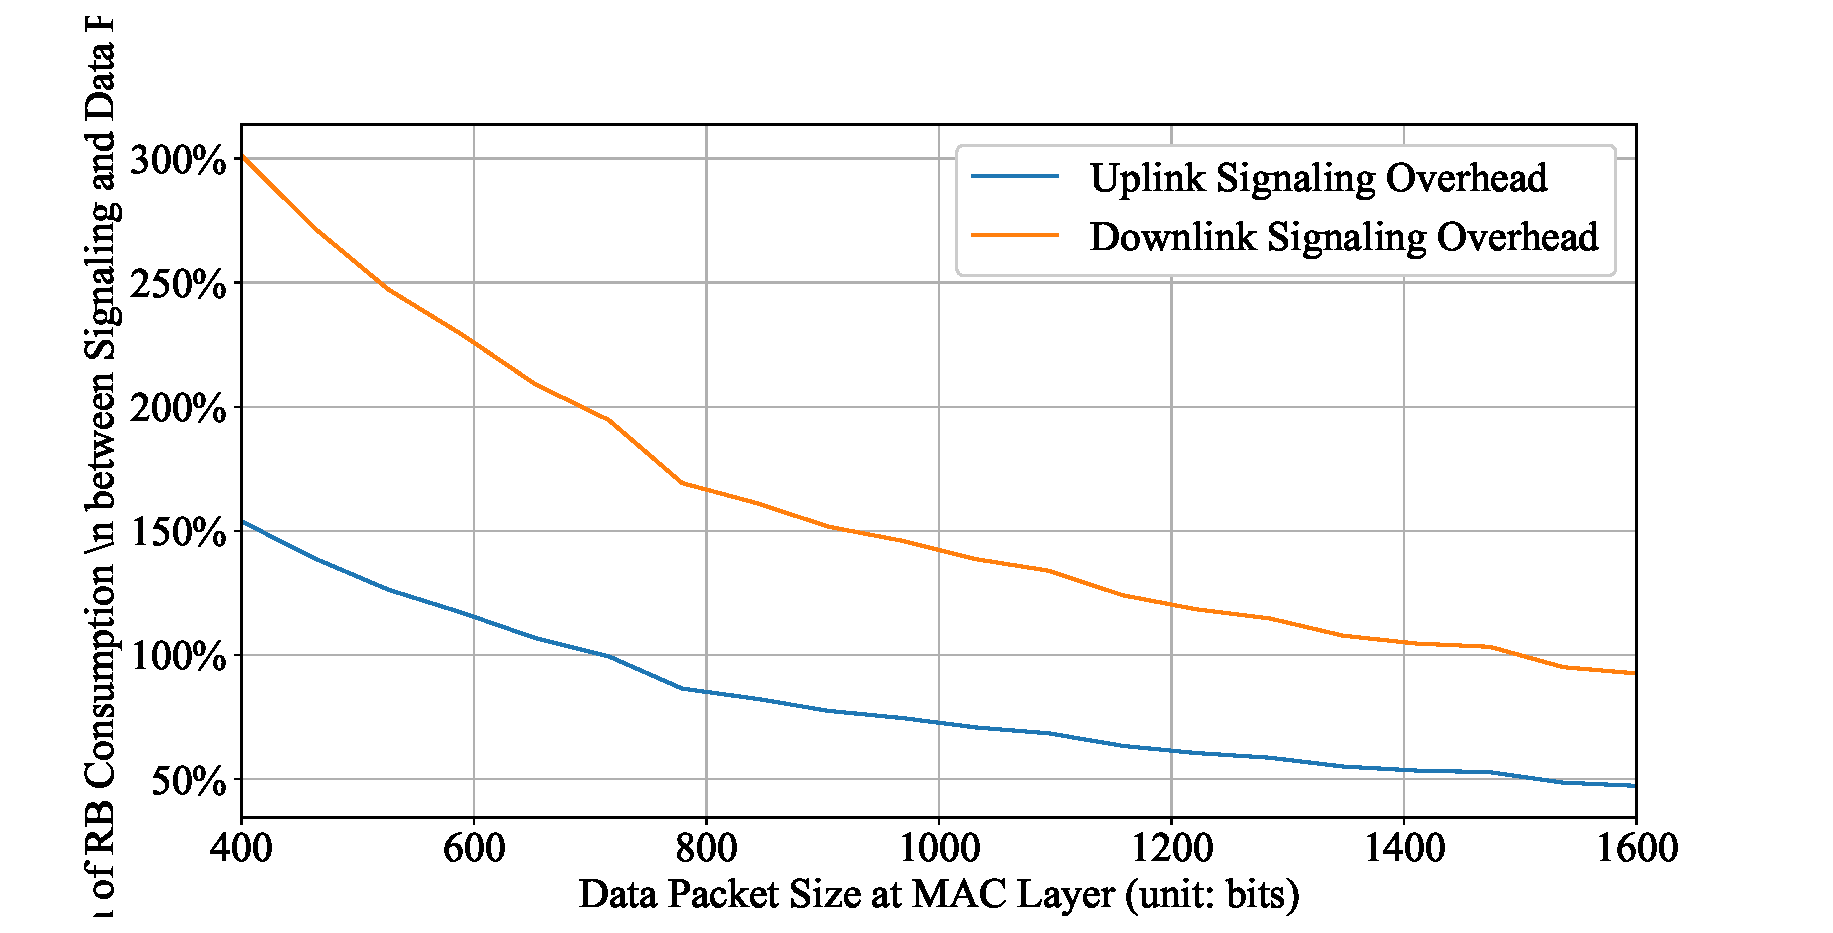
\includegraphics[width=\linewidth]{Chapter6/Figures/signaling_overhead_ratio.eps}
	\caption{Signaling overhead in terms of consumed RB number with respect to uplink reporting packet size}
	\label{fig:RB_signaling_overhead}
\end{figure}
By varying the packet size from $50$ bytes to $200$ bytes, the signaling overhead in terms of RB consumption is illustrated in Fig.~\ref{fig:RB_signaling_overhead}.

\begin{figure}[!t]
	\centering
	\includegraphics[width=\linewidth]{Chapter6/Figures/system_capa_occup_ratio.eps}
	\caption{ Average RB occupation ratio within a traffic model~\cite[Annex E]{3GPP/cellularIoT}}
	\label{fig:system_capa_occup_ratio}
\end{figure}

\subsection{Uplink Energy Efficiency Ratio}
We calculate the energy efficiency for our polling service and conventional LTE random access mechanism. The ratio between two methods are shown in Fig.~\ref{fig:energy_efficiency_ratio}.
We observe that the energy efficiency of our proposal is at least $1.15$ times of that in conventional LTE when data packet size is less than $600$ bits, the energy efficiency gain approaches to one with the augmentation of data packet size.

\begin{figure}[!t]
	\centering
	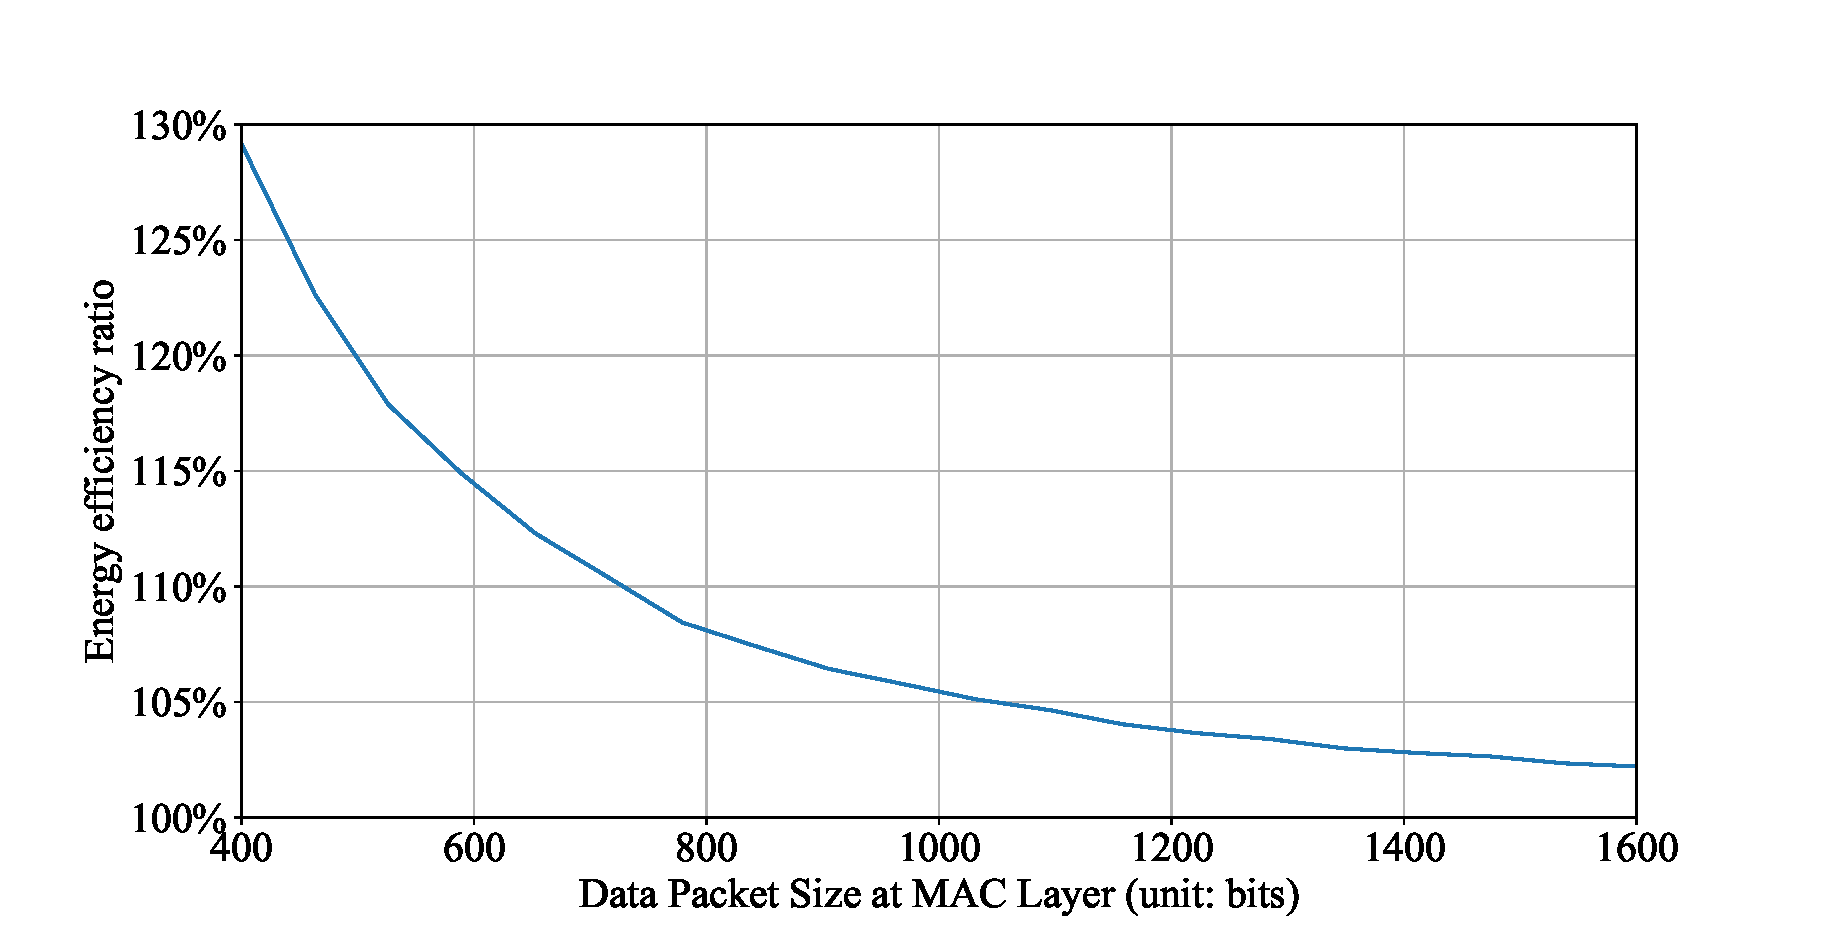
\includegraphics[width=\linewidth]{Chapter6/Figures/energy_efficiency_ratio.eps}
	\caption{Energy efficiency ratio with respect to uplink reporting packet size}
	\label{fig:energy_efficiency_ratio}
\end{figure}
% % Backup Text Zone
%Recall that MTC devices in conventional LTE networks should first attach to network before transmitting a $100$ bytes packets (MAC layer). Random access collision is not taken into account.

%Comparing Fig.~\ref{fig:lte-ra} and Fig.~\ref{fig:Comparison}, we observe that in the uplink direction data transmission with conventional random access should at least first send four signaling messages: random access preamble, RRC ConnectionRequest, RRC ConnectionSetupComplete and RRC ConnectionReconfigurationComplete while it requires zero message with our proposal. For the downlink direction, our proposal economizes the resources used for RAR, RRC ConnectionSetup, RRC ConnectionReconfiguration and RRC Connection release messages. That means that our proposal can effectively reduce signaling overhead for small payload and energy consumption. 
